\documentclass{beamer} %[handout]
\usetheme{CambridgeUS}
\usecolortheme{whale}
\usepackage{color}
\usepackage{xcolor}
\usepackage[makeroom]{cancel}
\usepackage{graphicx} 
\setbeamercolor{frametitle}{fg=black}
\usepackage{mathtools}
\usepackage{amssymb}
\usepackage{amsmath}
\usepackage{amsthm}
\usepackage{graphicx}
\usepackage{fancyvrb}
\usepackage{listings}
\usepackage{tikz}
\usepackage[utf8]{inputenc}

\usetikzlibrary{shapes}

\usetikzlibrary{decorations.text}

\lstset{frame=tb,
  language=R,
  aboveskip=3mm,
  belowskip=3mm,
  showstringspaces=false,
  columns=flexible,
  basicstyle={\tiny\ttfamily},
  numbers=none,
  numberstyle=\tiny\color{gray},
%  keywordstyle=\color{blue},
%  identifierstyle=\color{yellow},
  breaklines=true,
    literate={->}{$\rightarrow$}{2}
           {°}{$\epsilon$}{1},
  breakatwhitespace=true
  tabsize=3
}

\usetikzlibrary{arrows,positioning} 
\tikzset{
    %Define standard arrow tip
    >=stealth',
    %Define style for boxes
    punkt/.style={
           rectangle,
           rounded corners,
           draw=black, very thick,
           text width=6.5em,
           minimum height=2em,
           text centered},
    % Define arrow style
    pil/.style={
           ->,
           thick,
           shorten <=2pt,
           shorten >=2pt,}
}

\makeatletter
\def\th@mystyle{%
    \normalfont % body font
    \setbeamercolor{block title example}{bg=orange,fg=white}
    \setbeamercolor{block body example}{bg=orange!20,fg=black}
    \def\inserttheoremblockenv{exampleblock}
  }
\makeatother
\theoremstyle{mystyle}
\newtheorem*{remark}{Example}

\makeatletter
\def\th@mystylet{%
    \normalfont % body font
    \setbeamercolor{block title example}{bg=purple,fg=white}
    \setbeamercolor{block body example}{bg=purple!20,fg=black}
    \def\inserttheoremblockenv{exampleblock}
  }
\makeatother
\theoremstyle{mystylet}
\newtheorem*{analysis}{Example}

\date{}
\author[Bayesian statistics]{Erik \v{S}trumbelj\\2019}

\linespread{1.2}
\renewcommand{\thefootnote}{\roman{footnote}}
%\setbeameroption{show notes}

\begin{document}

\title[Multivariate Normal]{Exercise: Multivariate Normal model}

\begin{frame}
Bayesian statistics
\titlepage
\end{frame}

\begin{frame}
\begin{analysis}[Student grades]

\smallskip

\begin{minipage}[c]{0.33\linewidth}

\begin{center}
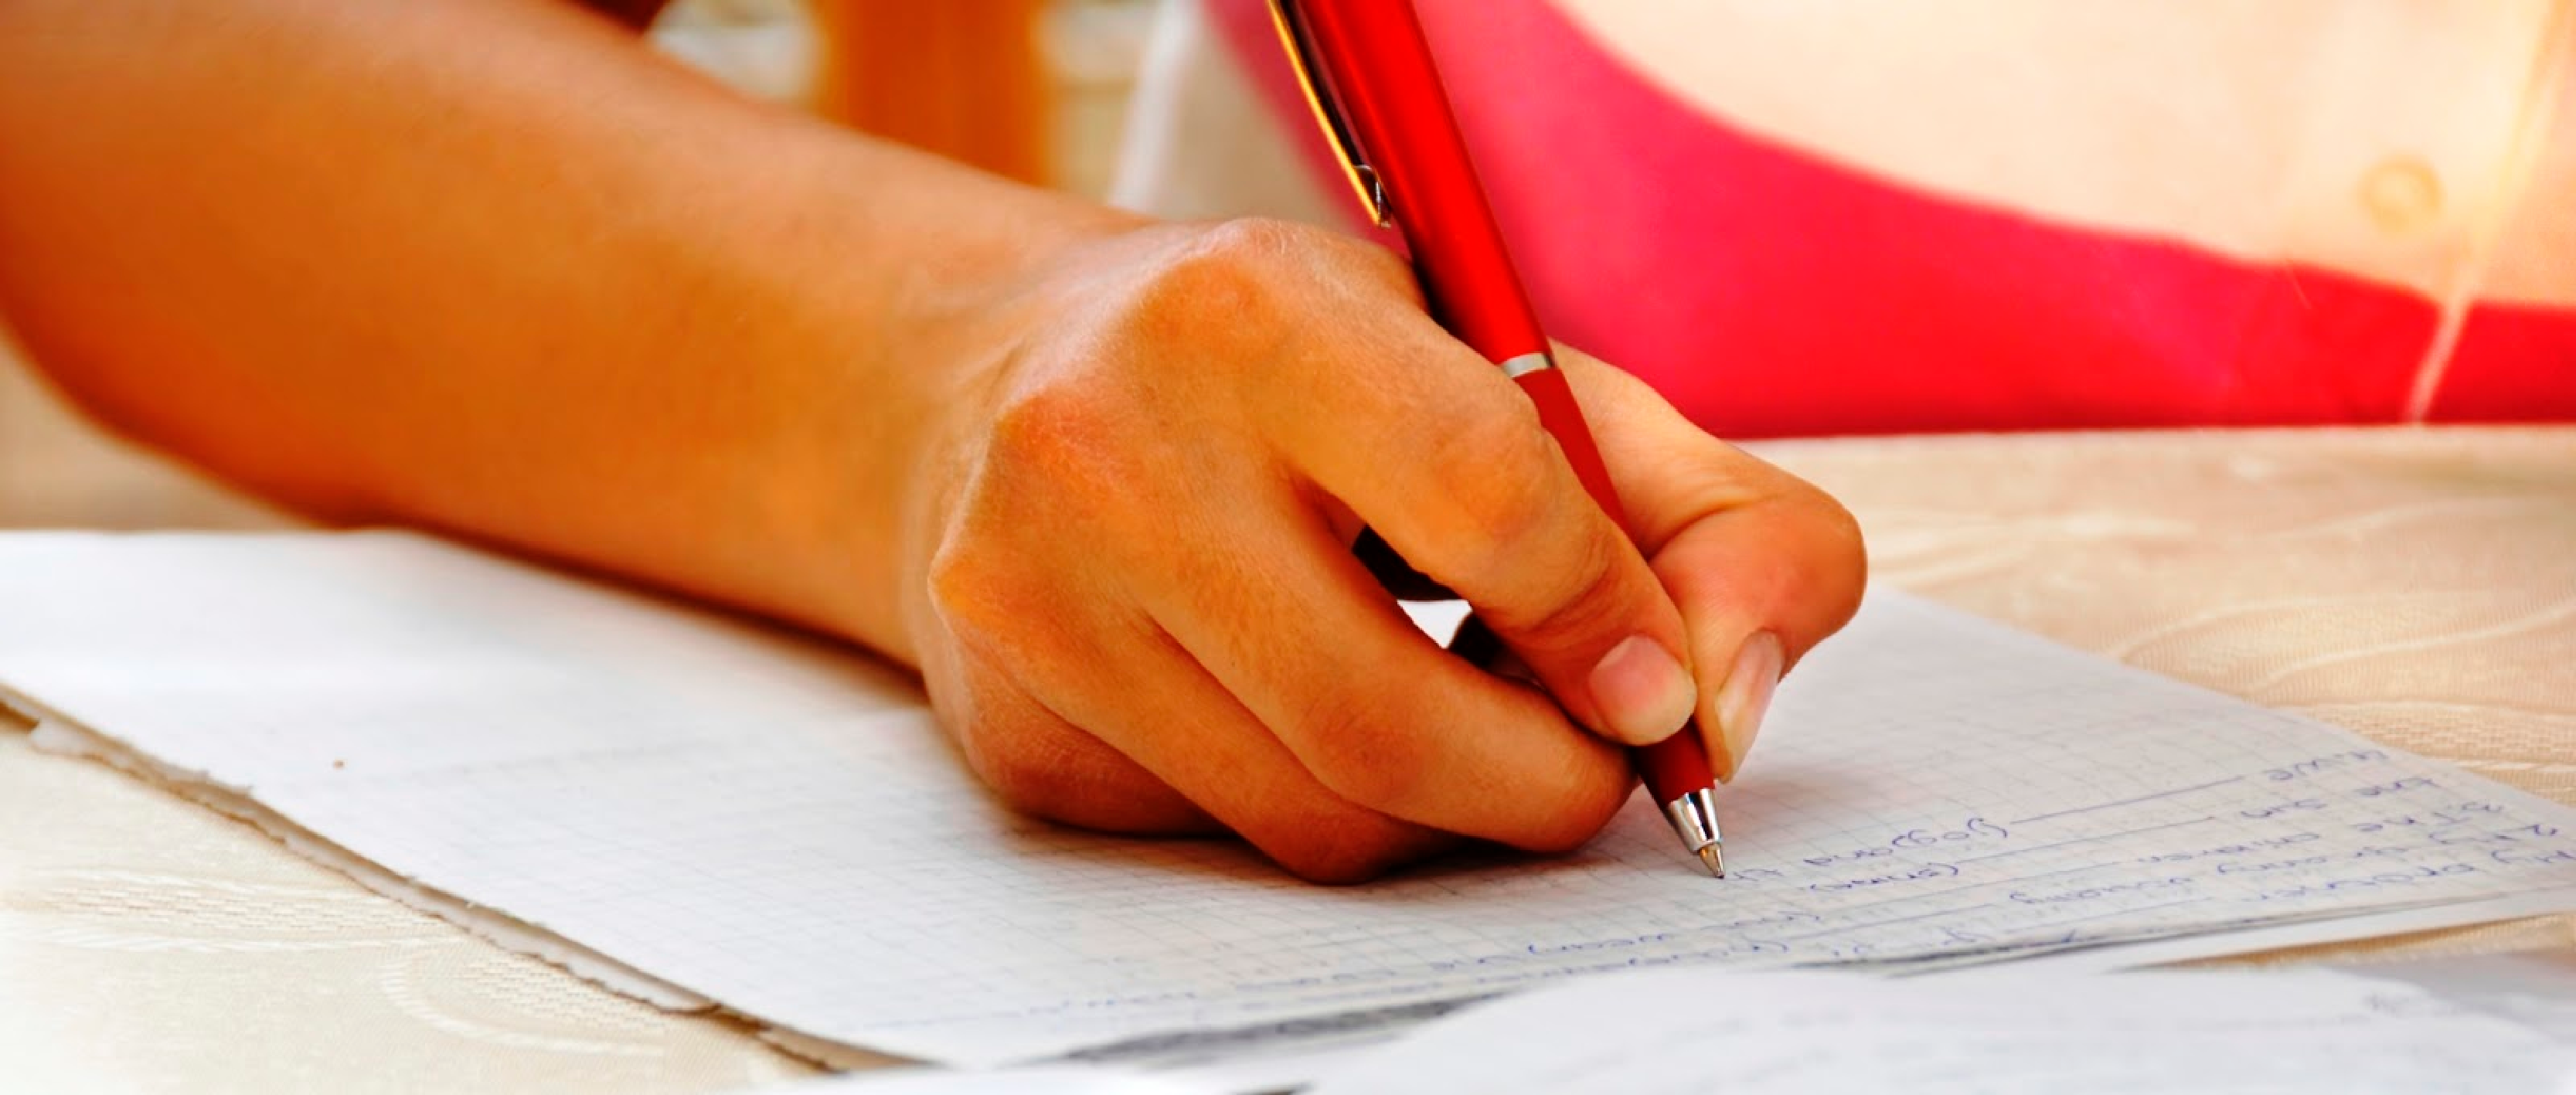
\includegraphics[width=1.0\linewidth]{../LectureAssets/L04/exam}
\end{center}

\begin{tiny}

\bigskip

100 students, 4 courses

\bigskip

\bigskip

Questions we are interested in:

\bigskip

\textbf{Which course is the most difficult?}

\bigskip

\textbf{Is Programming the easiest?}

\bigskip

\textbf{Are the math courses the most similar?}

\bigskip

\end{tiny}

\end{minipage} 
\begin{minipage}[c]{0.65\linewidth}

\begin{tiny}
\hfill\begin{tabular}{ccccc}
\hline
Student &  Calculus & Discrete math & Physics & Programming \\
\hline
1  &    8.0   &        7.0  &   6.5    &       7\\
2  &    6.5   &        6.0   &  6.0     &      7\\
3  &    8.0   &        8.0  &   6.5    &      10\\
4  &    7.5   &        7.5  &   7.0    &       7\\
5  &    6.0   &        6.5  &   6.0    &      10\\
6  &    7.5   &        8.0  &   8.0    &       8\\
... \\
\hline
\hline
\end{tabular}
\end{tiny}

\begin{center}
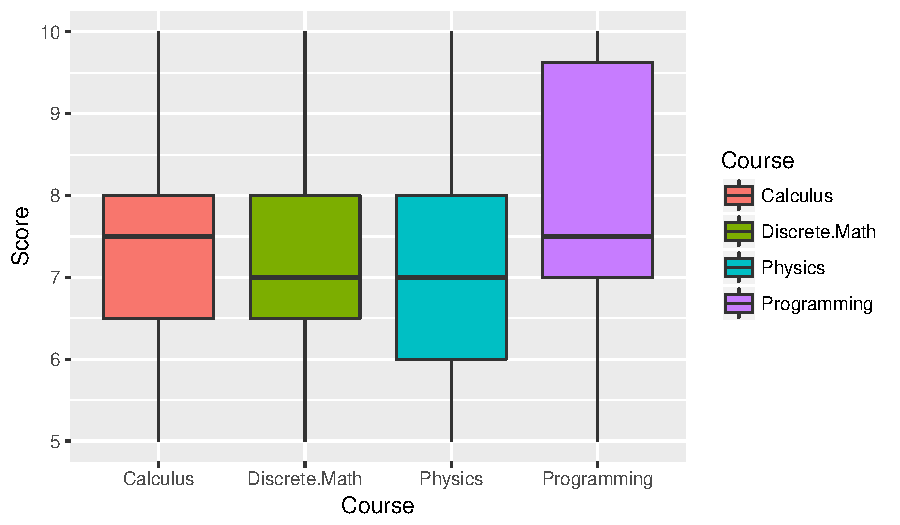
\includegraphics[width=0.80\linewidth]{../LectureAssets/L04/StudentScoresVis01}
\end{center}

\end{minipage}
\smallskip



\smallskip

\end{analysis}
\end{frame}

\begin{frame}{Two important questions}

\begin{Large}
Can we answer our questions with a model based on the Normal distribution (univariate or multivariate)? Should we use some other distribution instead?

\bigskip

\bigskip

\bigskip

Why use MVN distribution and not just use independent univariate Normal models (one for each course)?
\end{Large}
\end{frame}

\begin{frame}{Multivariate Normal (Gaussian) distribution}

Density of a k-variate Normal distribution:

$$p(\mathbf{y}) = \frac{1}{(2\pi)^{\frac{k}{2}}|\Sigma|^\frac{1}{2}} \exp\left[-\frac{1}{2}(\mathbf{y}-\mathbb{\mu})^T\Sigma^{-1}(\mathbf{y}-\mathbf{\mu})\right],$$

\bigskip

where data $\mathbf{y} = \begin{bmatrix} y_1 \\ \vdots \\ y_k
\end{bmatrix}$, mean vector $\mathbf{\mu} = \begin{bmatrix} \mu_1 \\ \vdots \\ \mu_k
\end{bmatrix}$, and covariance matrix $\Sigma = E[(\textbf{y} - \mu)(\textbf{y} - \mu)^T] = \begin{bmatrix} \sigma_1^2 & \sigma_{1,2} & \dots & \sigma_{1,k}\\ \sigma_{2,1} & \sigma_2^2 & \dots & \sigma_{2,k}\\ \vdots &  \vdots & \ddots & \vdots\\  \sigma_{k,1} & \sigma_{k,2} & \dots & \sigma_k^2
\end{bmatrix}$.

\bigskip

Any restrictions regarding $\mu$ or $\Sigma$?

\end{frame}

\begin{frame}{Bayesian MVN model}

\begin{small}
\textbf{Model }(likelihood), use reparametrization $\Lambda = \Sigma^{-1}$:

$y_i|\mu, \Lambda \sim MVN_k(\mu, \Lambda^{-1})$

\smallskip

\textbf{Conjugate prior:}

$\mu | \Lambda \sim MVN_k(\mu_0, (\kappa_0\Lambda)^{-1})$

$\Lambda \sim \text{Wishart}(\nu, S_0)$

\smallskip

\textbf{Posterior:}

$\mu | \pmb y, \Lambda \sim MVN_k(\mu_n, (\kappa_n\Lambda)^{-1})$

$\Lambda | \pmb y \sim \text{Wishart}(\nu_n, S_n^{-1})$

$\mu_n = \frac{\kappa_0\mu_0 + n\overline{y}}{\kappa_0 + n}$

$\kappa_n = \kappa_0 + n$

$S_n = S_0 + \sum_{i = 1}^n (y_i - \overline{y})(y_i - \overline{y})^T + \frac{\kappa_0 n}{\kappa_0 + n}(\mu_0 - \overline{y})(\mu_0 - \overline{y})^T$

$\nu_n = \nu_0 + n$
\end{small}
\end{frame}

\end{document}
